%!TEX root=../oi-magistr-si.tex
\section[TPJ - sémantiky: operační, denotační]{Sémantika: operační sémantika, denotační sémantika, pevný bod funkce, vázání jmen, stav programu a data.}

\noindent Sémantika programovacích jazyků je v teorii programovacích jazyků \textbf{obor} zabývající se \textbf{důsledným matematickým popisem významu} programovacího jazyka \cite{wiki:semantika}.

\noindent 3 hlavní charakteristiky jazyka jsou: 

\begin{itemize}[itemsep=0px]
\item \textbf{syntaxe} se zabývá formou (znaky a jejich vztahy),
\item \textbf{sémantika} významem znaků,
\item \textbf{pragmatika} závislostí konstrukcí na nositeli - implementace.
\end{itemize}

\textbf{Operační sémantika} je \textbf{přístup}, který \textbf{definuje sémantiku} programovacího jazyka tak, že určí jak je libovolný program vykonán na počítači, jehož činnost je známa. Může to být nějaký abstraktní stroj, který je dostatečně jednoduchý pro snadné pochopení jeho činnosti (například Turingův stroj). Operační sémantika potom specifikuje, jak tento stroj zpracovává program v definovaném jazyku.

\paragraph{Operační exekuce}

\begin{itemize}[itemsep=0px]
\item Program + vstupy $\rightarrow$ Vstupní funkce
\item Iniciální konfigurace
\item (Mezikonfigurace ...)
\item Finalní konfigurace
\item Výstupní funkce $\rightarrow$ Odpověď
\end{itemize}

\subsection{Sémantika malého kroku (SOS)}
\begin{itemize}[itemsep=0px]
\item Definujeme přepisovací relaci $\Rightarrow \in Expr \times Expr$.
\item Výraz $e \Rightarrow e'$ znamená, že přepis $e$ na $e'$ je vykonán v jednom kroku.
\end{itemize}

\paragraph{Formální definice} $S = \langle CF,\Rightarrow, FC, IF, OF \rangle$

\begin{itemize}[itemsep=0px]
\item CF – doména konfigurací (obor hodnot)
\item $\Rightarrow$ – přepisovací relace (transformuje konfigurace) ($\Rightarrow \subseteq CF \times CF$)
\item FC – množina finálních konfigurací (nezjednodušitelné konfigurace) ($FC\subseteq CF$)
\item IF – vstupní funkce $(\text{Prog} \times \text{Inputs}) \rightarrow CF$.
\item OF – výstupní funkce $FC \rightarrow \text{Answer}$
\end{itemize}

\paragraph{Pravidla} $e,e_1,e_2,e' \in Expr \quad n,n' \in Num$

$$\frac{}{\bigtriangleup n \Rightarrow -n}$$

$$\frac{}{n \odot n' \Rightarrow n + n'}$$

$$\frac{e \Rightarrow e'}{e \bigtriangleup \Rightarrow \bigtriangleup e'}$$

$$\frac{e_1 \Rightarrow e'}{e_1 \odot e_2 \Rightarrow e' \odot e_2}$$

$$\frac{e_2 \Rightarrow e'}{e_1 \odot e_2 \Rightarrow e_1 \odot e'}$$

\subsection{Sémantika velkého kroku (BOS)}
\noindent Odlišný přístup než SOS. Program je vyhodnocen v jednom kroku. Zde je definována přepisovací relace

$$\Longrightarrow \in Expr \times Num$$

\paragraph{Pravidla} $e,e_1,e_2 \in Expr \quad n,n_1,n_2 \in Num$

$$\frac{}{n \Longrightarrow n}$$

$$\frac{e \Longrightarrow n}{\bigtriangleup e \Longrightarrow -n}$$

$$\frac{e_1 \Longrightarrow n_1 \quad e_2 \Longrightarrow n_2}{e_1 \odot e_2 \Longrightarrow n_1 + n_2}$$

\example{Příklad SOS (jedno z možných vyhodnocení):}{
    \begin{spacing}{0}
    $$
    \cfrac{
        \cfrac{
            \cfrac{}{
                \bigtriangleup 15 \Rightarrow -15
            }
        }{
        (\bigtriangleup 15) \odot (\bigtriangleup 24) \Rightarrow -15 \odot (\bigtriangleup 24)
        }
    }{
        \bigtriangleup((\bigtriangleup 15) \odot (\bigtriangleup 24)) \Rightarrow \bigtriangleup(-15 \odot (\bigtriangleup 24))
    }$$
    \end{spacing}
    \vspace{20px}
}

\example{Příklad BOS:}{
    \begin{spacing}{0}
    $$
    \cfrac{
        \cfrac{
            \cfrac{
                \cfrac{}{
                    15 \Longrightarrow 15 \quad 24 \Longrightarrow 24
                }
            }{
                \bigtriangleup 15 \Longrightarrow -15 \quad \bigtriangleup 24 \Longrightarrow -24
            }
        }{
        (\bigtriangleup 15) \odot (\bigtriangleup 24) \Longrightarrow -15 + -24
        }
    }{
        \bigtriangleup((\bigtriangleup 15) \odot (\bigtriangleup 24)) \Longrightarrow -(-15 + -24)
    }$$
    \end{spacing}
    \vspace{20px}
}



\subsection{Denotační sémantika}

Denotační sémantika používá k popisu sémantiky programovacího jazyka funkce. Tyto funkce přiřazují sémantické hodnoty správným syntaktickým zápisům. Příkladem může být funkce Val, která přiřadí výrazu jeho hodnotu:

$$\text{Val}: \text{Výraz} \rightarrow \text{Integer}$$

Doménou syntaktických funkcí se nazývá syntaktická doména - u funkce Val je to množina všech správných aritmetických výrazů. Obor hodnot je sémantická doména - zde množina celých čísel. Denotační definice jazyka má tedy 3 části - syntaktickou doménu, sémantickou doménu a definici jednotlivých funkcí.

\begin{itemize}[itemsep=0px]
\item \textbf{Syntaktická algebra} - popisuje abstraktní syntaxy jazyka, může být specifikována gramatikou.
\item \textbf{Sémantická algebra} - modeluje význam frází, skládá se z kolekce sémantických domén.
\item \textbf{Významová funkce} - mapuje elementy syntaktické algebry k jejich významu v sémantické algebře. Funkce musí být homomorfismus mezi syntaktickou a sémantickou algebrou.
\end{itemize}

\subsubsection{Významová funkce (Meaning function)}
Uvažujte $M$ jako významovou funkci a $t$ je prvek v abstraktním syntaktickém stromu s potomky $t_1, \hdots, t_k$. Pak

$$(M t) = (f_t (M t_1) \hdots (M t_k))$$

kde $f_t$ je funkce určená syntaktickou třídou.

\begin{figure}[h!]
\centering
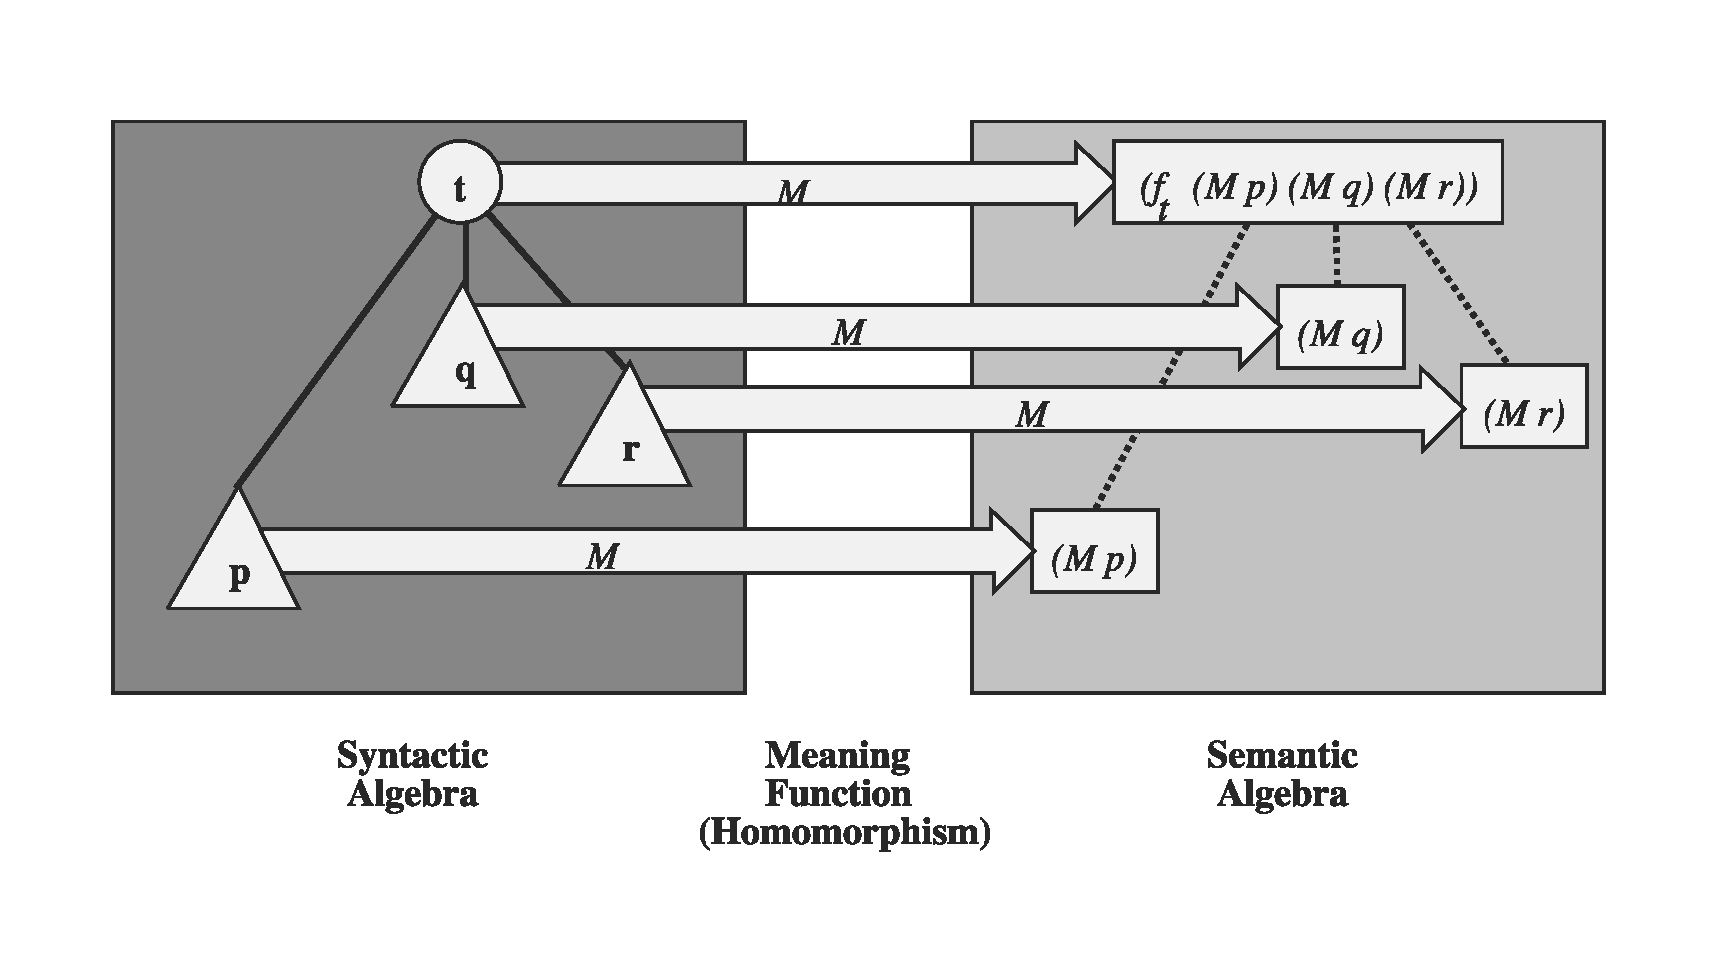
\includegraphics[width=125mm]{01/images/tpj-homo}
\end{figure}

\paragraph{Denotační sémantika} $Expr $ ::= $ Num \quad | \quad \bigtriangleup Expr \quad | \quad Expr \odot Expr$

\noindent Sémantická doména $N$

$$[\![n]\!] = n$$

$$[\![\bigtriangleup e]\!] = [\![\bigtriangleup]\!]([\![e]\!])$$

$$[\![\bigtriangleup]\!] = \lambda x.-x \quad \text{(např. unární mínus)}$$

$$[\![e_1 \odot e_2]\!] = [\![\odot]\!]([\![e_1]\!], [\![e_2]\!])$$

$$[\![\odot]\!] = \lambda x,y.x+y \quad \text{(např. plus)}$$

\subsection{Pevný bod funkce}
Jako pevný bod označujeme bod, který se v daném zobrazení zobrazí sám na sebe. Označuje se také jako samodružný bod. Například pevnými body funkce $f(x)=x^2-4x+6$, jsou čísla 2 a 3.

\begin{itemize}
\item bod, ve kterém platí $f(x) = x$
\item využívá se pro rekurzivní funkce
\item Y kombinátor v lambda kalkulu: \texttt{Y = $\lambda$y($\lambda$x.y(xx))($\lambda$x.y(xx))}
\end{itemize}

\priklad
Generující funkce faktoriálu fact = \texttt{$\lambda$F.$\lambda$X.if x==0 then 1 else F(decrement(X))}. Generující funkci dám do Y kombinátoru:

\begin{lstlisting}[
  mathescape,
  columns=fullflexible,
  basicstyle=\fontfamily{lmvtt}\selectfont,
]
Y fact =
       = $\lambda$f ($\lambda$x.y(xx))($\lambda$x.y(xx)) fact =
       = ($\lambda$x.fact(xx))($\lambda$x.fact(xx)) =
       = fact( ($\lambda$x.fact(xx) ($\lambda$x.fact(xx) ) =
       = fact(Y fact)
\end{lstlisting}

\noindent \texttt{Y fact} je pevný bod funkce, která počítá faktoriál.

\subsection{Vázání jmen}
Vázání jmen se vyskytuje v lambda kalkulu.
\paragraph{$\lambda$-kalkul} Je formální popis, který slouží jako základ pro funkcionální jazyky, takže všechny konstrukce v těchto jazycích jdou přepsat právě na $\lambda$-kalkul. Základní prvky $\lambda$-kalkulu jsou tři následující:
\begin{itemize}
\item \textbf{Proměnné} Obyčejné proměnné, tak jak je znáte z jiných jazyků, většinou se značí \texttt{x,y,z}.

\item \textbf{Abstrakce} Definice funkce – představte si např. funkci \texttt{f(x) = x+2}, tak přesně taková funkce se v $\lambda$-kalkulu zapíše takto: \texttt{$\lambda$x.x+2}. Část mezi $\lambda$ a tečkou jsou parametry funkce (zde máme pouze jeden parametr) a za tečkou se nachází tělo funkce.

\item \textbf{Aplikace} Volání funkce – když si vezmu naši funkci \texttt{f(x) = x+2}, tak ta se zavolá např. s argumentem 3 takto: \texttt{f(3)}. Funkce v $\lambda$-kalkulu se volají podobně, funkce se volá takto: \texttt{(f 3)}, tzn. nejdříve je uvedena funkce a poté její argumenty. Funkce f se v $\lambda$-kalkulu tedy zavolá takto: \texttt{($\lambda$x.x+2) 3}. Vysvětlení by mělo být už jasnější. Číslo 3 se dosadí za parametr \texttt{x} a přejde se do těla funkce, tam se ke 3 přičte 2 a výsledkem je 5.
\end{itemize}

\noindent Proměnná je v $\lambda$-výrazu \textit{vázaná}, pokud se jedná o parametr nějaké funkce, takže např. ve výrazu (\texttt{$\lambda$x.yx}) je \texttt{x} vázaná proměnná. Ostatní proměnné (v minulém příkladu \texttt{y}) jsou \textit{volné}. Proměnná se vždycky váže na nejbližsí lambdu vlevo, takže ve výrazu \texttt{($\lambda$x(($\lambda$x.x) w))} se proměnná \texttt{x} uprostřed výrazu váže na lambdu co je hned vlevo od ní a ne na tu úplně vlevo! Proměnná \texttt{w} je samozřejmě volná \cite{lambda}.

\begin{itemize}
\item Funkce, co mají jen vázané proměnné, vrátí při každém zavolání stejný výsledek. Funkce s volnými proměnnými jsou závislé na globálním kontextu.
\item Funkce, co mají jen vázané proměnné, se v $\lambda$-kalkulu nazývají kombinátory.
\end{itemize}

$$\texttt{(}\lambda\texttt{x.xy)}$$

$$\texttt{(}\lambda\texttt{x.x)(}\lambda\texttt{y.yx)}$$

\subsection{Stav programu}
Stav = proměnné v prostředí, proměnné mají typ, prostředí = množina všech proměnných, kontext (v handoutech $\Gamma$ (Gamma))
Čistě funkční jazyky (a matematika) jsou bezestavové, stavové výpočty mohou být reprezentovány jako iterace skrz stavy.

Čistě funkční jazyky (a matematika) jsou bezestavové, stav může být modelován jako iterace skrz stavy.
\example{Funkce na nalezení maxima z pole:}{
$$max:N* \rightarrow N$$

$$max(\langle a_1, \hdots, a_n \rangle) = loop(\langle a_1, \hdots, a_n \rangle,1,0)$$

$$loop: N* \times N \times N \rightarrow N$$

$$loop(\langle a_1, \hdots, a_n \rangle,c,m) = m \qquad \text{if} \quad c > n$$

$$loop(\langle a_1, \hdots, a_n \rangle,c,m) = loop(\langle a_1, \hdots, a_n \rangle,c+1,m) \qquad \text{if} \quad c \leq n \wedge a_c \leq m$$

$$loop(\langle a_1, \hdots, a_n \rangle,c,m) = loop(\langle a_1, \hdots, a_n \rangle,c+1,a_c) \qquad \text{otherwise}$$

\vspace{20px}
}

\paragraph{Monády} - struktury (typy), co reprezentují výpočet jako sekvenci kroků.

\subsection{Data programu}
Dělí se na \textbf{součiny}, \textbf{sumy} a \textbf{sumy součinů}.

\begin{itemize}[itemsep=0px]
\item Součiny
\begin{itemize}[itemsep=0px]
\item Positional data = N-tice, každý prvek může mít jiný typ
\item Sequence, List = pole
\item Named = třída
\item Nonstrict, stream = data, která se získají/vypočítají v okamžiku, kdy je potřeba (např. InputStream, odněkud se to vezme)
\end{itemize}

\item Sumy - Union v C, nadtypy v Javě.
\item Sumy součinů - Binární a ternální operátory, double dispatch.
\end{itemize}